\documentclass[10pt]{amsart}
\usepackage[T1]{fontenc}
\usepackage{beton}
\usepackage{euler}
\usepackage{latexsym}
\usepackage{amsmath}
\usepackage{amssymb}
\usepackage{amsthm}
\usepackage{epsfig}

\newcommand{\C}{{\mathbb  C}}
\newcommand{\R}{{\mathbb  R}}
\newcommand{\Z}{{\mathbb  Z}}
\newcommand{\N}{{\mathbb  N}}
\newcommand{\Q}{{\mathbb  Q}}

\makeatletter
\renewcommand{\leq}{\leqslant}
\renewcommand{\geq}{\geqslant}
\renewcommand{\Re}{{\operator@font Re\,}}
\renewcommand{\Im}{{\operator@font Im\,}}
\makeatother

\newtheorem{lemma}{Lemma}

\renewcommand{\ttdefault}{pcr}

\frenchspacing

\begin{document}

\title{Taming a Hydra of Singularities}
\author{Folkmar Bornemann and Thomas Schmelzer}
\keywords{} \subjclass{}
\thanks{July 24, 2005}
\maketitle

\section{Introduction}
\noindent
We invite the reader to contemplate for one moment the following remarkable limit problem
(where $g^{[n]} = g \circ g \circ \cdots \circ g$ denotes the $n$-fold iteration of a function $g$):

\bigskip

\begin{quote}{\em
Consider a function $f: \R \to \R$ that is bounded and continuous. Does the sequence of violently oscillatory integrals
\[
\frac{1}{\pi}\int_0^\pi f(\tan^{[n]}x)\,dx, \qquad n=1,2,3,\ldots,
\]
have a limit as $n$ approaches infinity? If so, what is the limit?}
\end{quote}

\medskip

\begin{figure}[hb]
\begin{center}
\hspace*{-0.5mm}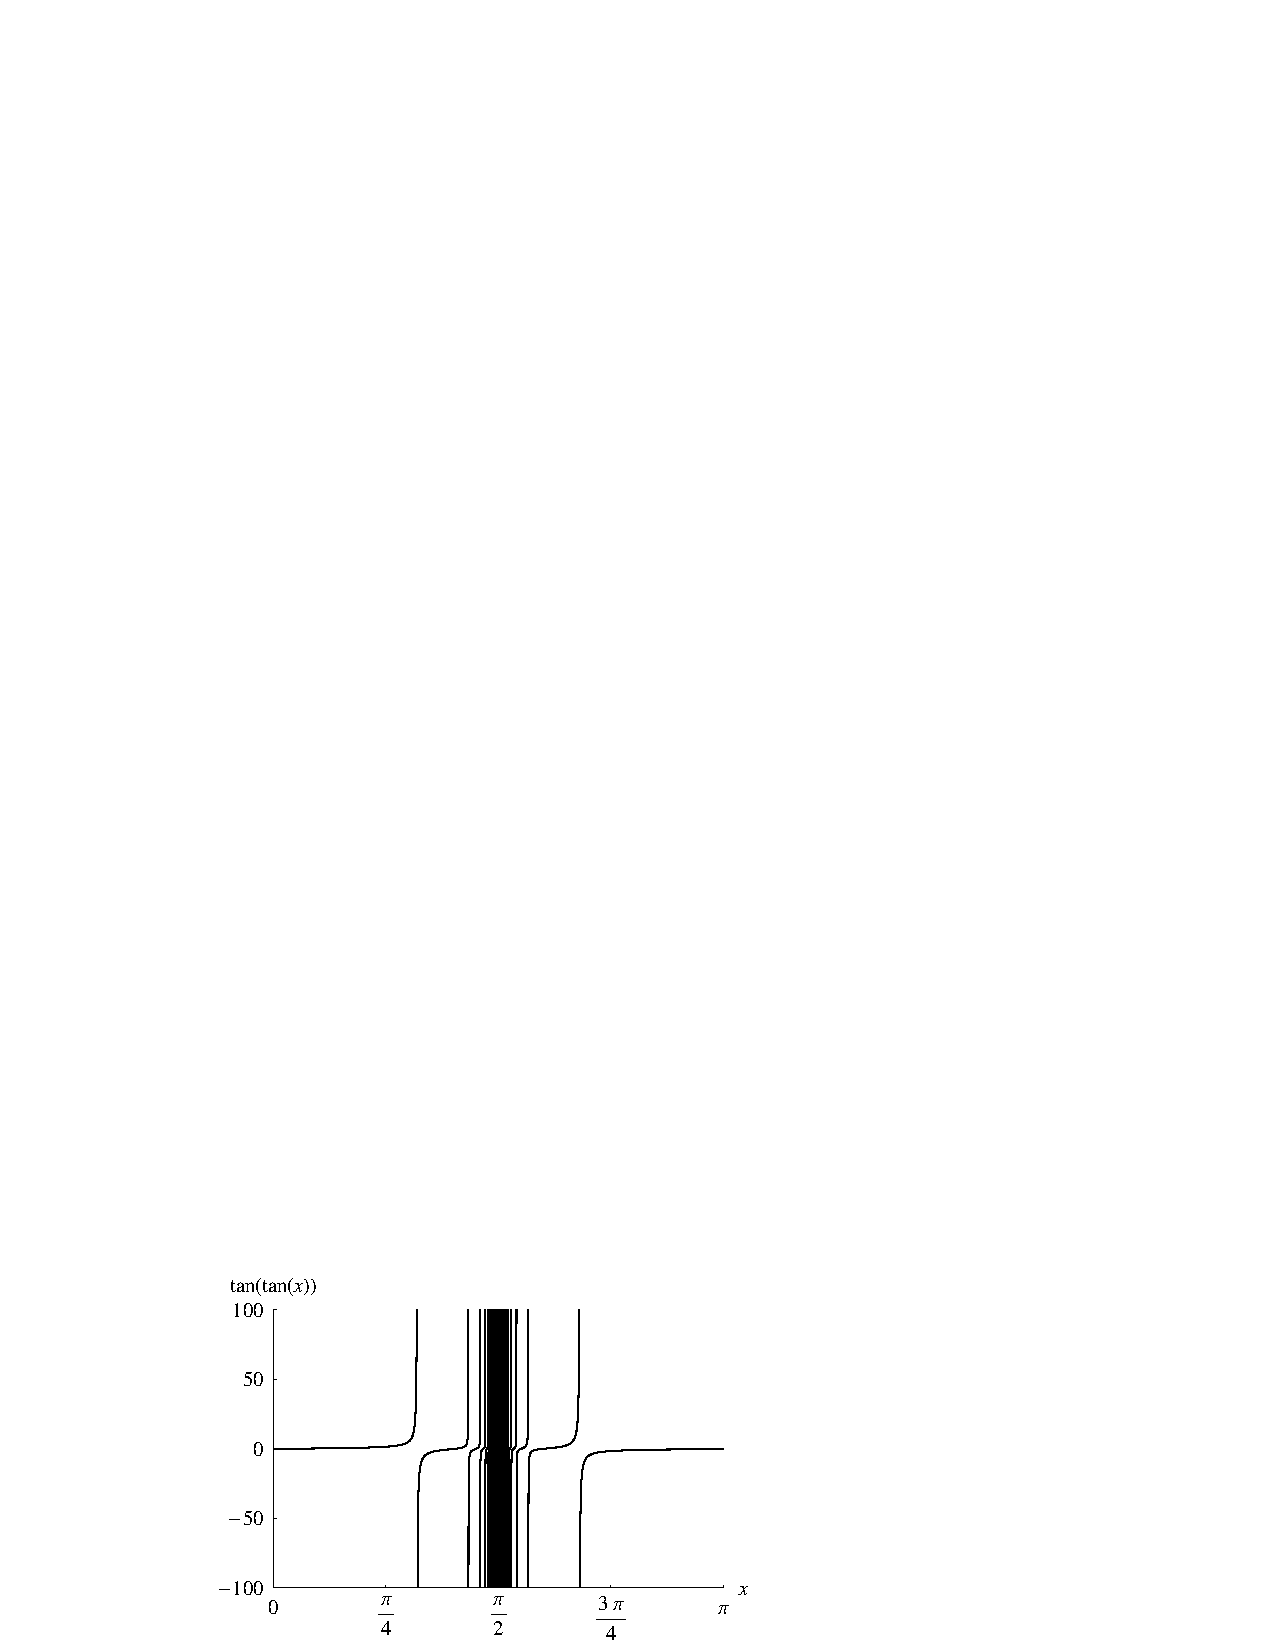
\includegraphics[scale=0.668]{tan2.pdf}\;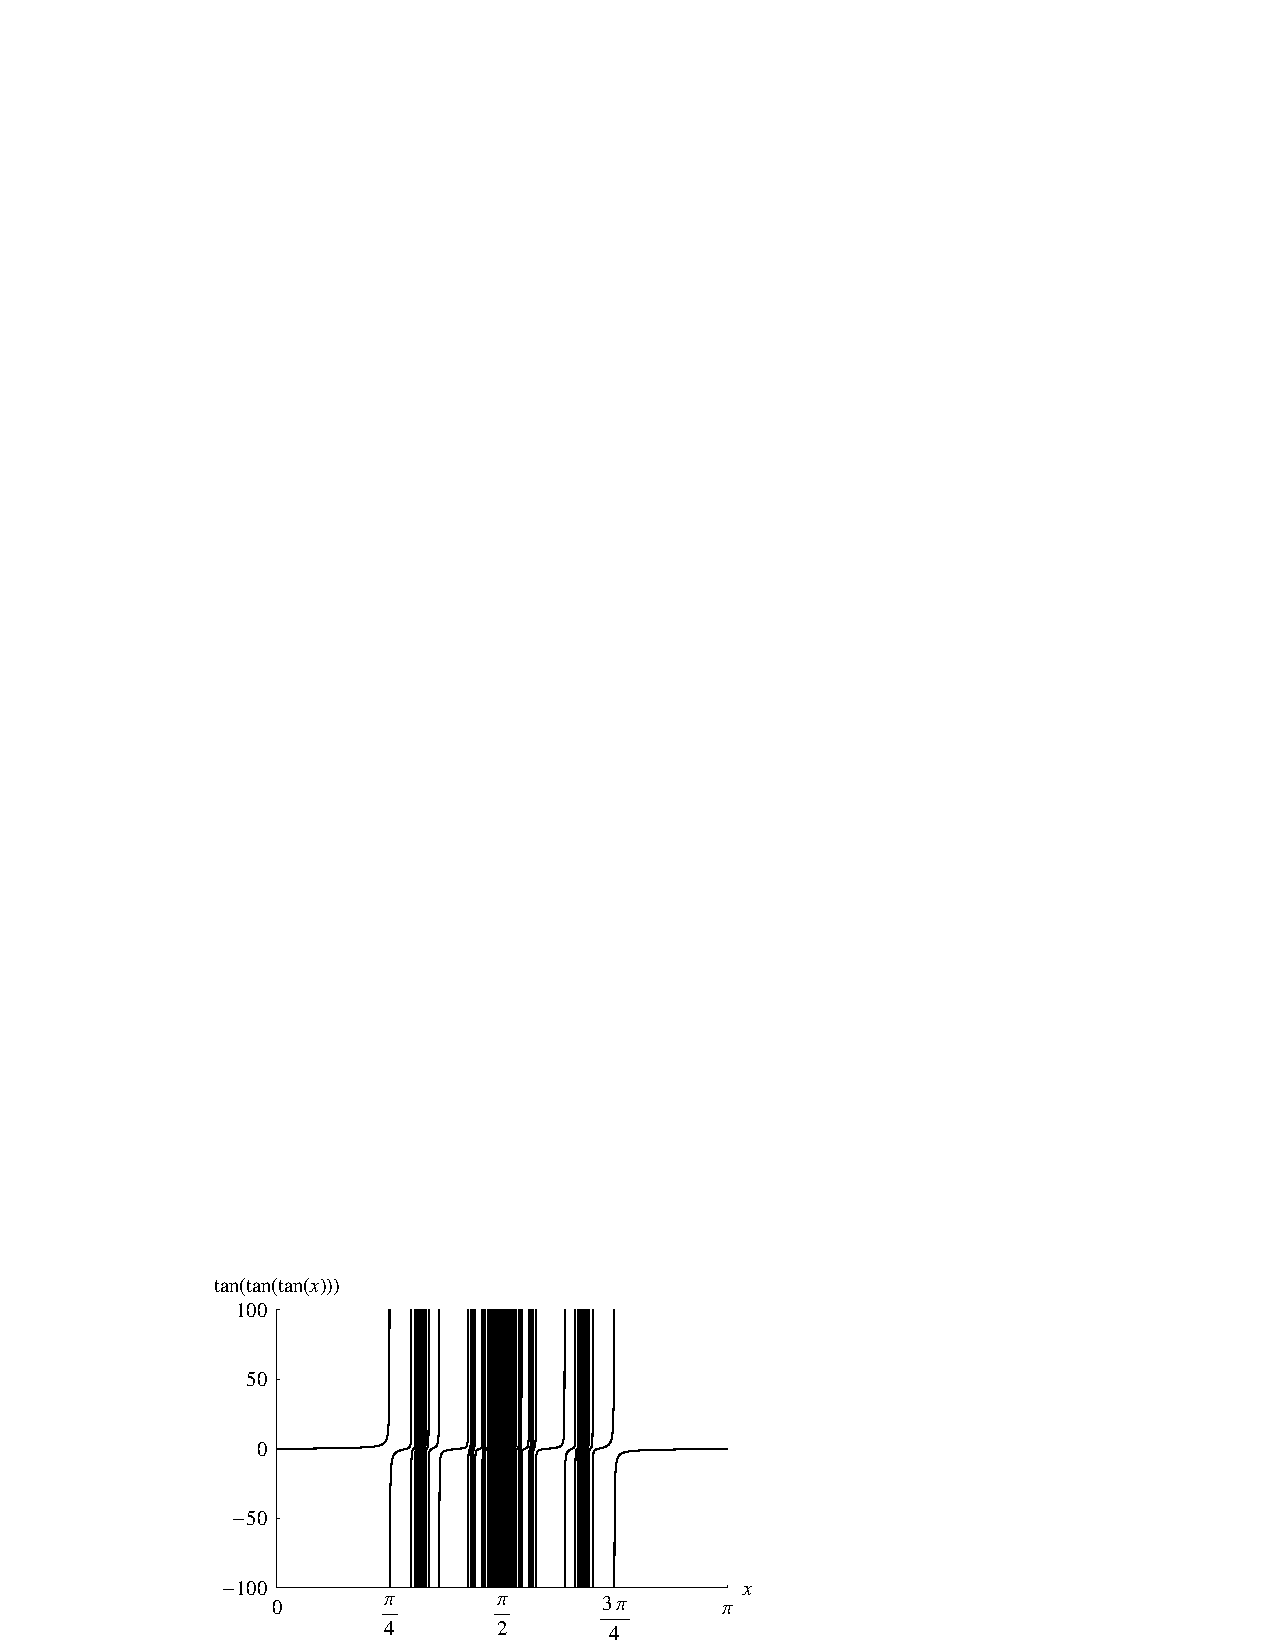
\includegraphics[scale=0.668]{tan3.pdf}
\end{center}
\caption{Graph of  $\tan^{[2]}(x)$ (left) and $\tan^{[3]}(x)$ (right).}
\end{figure}
%
\noindent
Figure~1 gives just a faint impression of the Herculean drama caused by the iterated function $\tan^{[n]}(x)$. Starting with the singularities
of $\tan(x)$ at $x=(k+1/2)\pi$, $k \in \Z$, each singularity of the $n$-fold iteration $\tan^{[n]}(x)$
breeds like the mythic Hydra countably many new singularities for the next iteration $\tan^{[n+1]}(x)$, which accumulate in their respective ancestor.
As $x$ moves from one singularity to the next, the values of $\tan^{[n]}(x)$  go all the way from $-\infty$ to $+\infty$. Asymptotically,
as $n\to\infty$, these proliferating singularities become \emph{dense} in $[0,\pi]$.

So, having this desolate picture in mind, what would possibly be a reasonable guess about the destiny of the limit of the integrals?

If we were more gentle and put $\tanh$ in place of $\tan$, the problem would allow for an easy solution. In fact,
we would then have the inequality $0 < \tanh x<x$ and therefore the monotone limit
\begin{equation}\label{eq.tanh}
\lim_{n\to\infty} \tanh^{[n]} x = 0,\qquad x>0.
\end{equation}
Hence, by dominated convergence, using the boundedness and continuity of $f$ we would obtain asymptotic focussing to the value of $f$ at zero,
\[
\lim_{n\to\infty} \frac{1}{\pi}\int_0^\pi f(\tanh^{[n]}x)\,dx = \frac{1}{\pi}\int_0^\pi f(\lim_{n\to\infty} \tanh^{[n]}x)\,dx = \frac{1}{\pi}\int_0^\pi f(0)\,dx = f(0).
\]
Quite on the contrary, we have $\lim_{n\to\infty} \tan^{[n]} x = 0$ just for countably many $x$, that is, for a negligible set
of measure zero. Generically in $x$, the sequence $\tan^{[n]} x$ oscillates violently as $n \to \infty$, thereby taking values that are widely spread in
$(-\infty,\infty)$.
One might thus expect that the integrals would, if at all, converge to some averaged value of $f$.

However, in this note we will prove, based on unexpectedly explicit evaluations of the involved integrals,
that the limit is, quite remarkably, exactly in the same way focussing to the value of $f$ at zero,
\begin{equation}\label{eq.claim}
{\lim_{n\to\infty}\frac{1}{\pi}\int_0^\pi f(\tan^{[n]}x)\,dx = f(0).}
\end{equation}
To begin with, let us briefly explain why the integrals of the sequence exist. Because $\tan^{[n]} x$ is defined a.e.~on $[0,\pi]$ (with the exception of the proliferated, countably many
singularities already discussed), the integrand $f(\tan^{[n]} x)$ is bounded and continuous a.e.; therefore,
it is (Riemann) integrable.

\section{A First Proof: Potential Theory}
\noindent
We set the scene with some heavier theoretical machinery; an elementary proof that does not
rely on complex analysis will be given later on. Throughout this note we assume that $f:\R \to \R$ is bounded and continuous.
Now, from potential theory (see \cite[Thms. 15.1a, 15.4d]{Hen}) we know that there is a function $F(z)$, holomorphic
in the upper complex half plane $\Im z >0$, such that the harmonic function $\Re F(z)$ is bounded and has boundary values given by $f$, that is,
\begin{equation}\label{eq.F}
\Re F(x+ i y) \to f(x), \qquad x\in\R,
\end{equation}
as the real number $y$ approaches zero from above. The holomorphic function $F$ is \emph{unique}
up to a purely imaginary additive constant. For the sake of simplicity of our presentation, we will further
{\em assume that $F$ itself, not just $\Re F$, is bounded}\/; this additional assumption will be dropped
in the elementary, real analysis proof of Section~\ref{sect.real}, which  will also show that the identities (\ref{eq.Qexpl}) and (\ref{eq.real})
remain valid then.


The substitution $\xi = \tan(x)$ transforms the integral as
\begin{equation}\label{eq.trans}
\frac{1}{\pi} \int_0^\pi f(\tan^{[n+1]}x)\,dx = \frac{1}{\pi} \int_{-\infty}^\infty \frac{f(\tan^{[n]}\xi)}{1+\xi^2}\,d\xi.
\end{equation}
By (\ref{eq.F}), by the boundedness of $F$, and by the fact that $\tan(z)$ maps the upper complex half plane into itself, we get using dominated convergence
\begin{multline}\label{eq.limit}
\frac{1}{\pi} \int_0^\pi f(\tan^{[n+1]}x)\,dx = \frac{1}{\pi} \int_{-\infty}^\infty \frac{f(\tan^{[n]}\xi)}{1+\xi^2}\,d\xi \\
= \lim_{\epsilon\downarrow 0} \Re \frac{1}{\pi} \int_{-\infty}^\infty \frac{F(\tan^{[n]}(\xi+i\epsilon))}{1+(\xi+i\epsilon)^2}\,d\xi.
\end{multline}
Let us fix an $0 < \epsilon < 1$. For $R>1$ we denote by $\mathcal{C}_R$ the boundary of the half-circle with center $i\epsilon$ that connects $-R+i\epsilon$ through
$i(R+\epsilon)$ with $R+i\epsilon$. Cauchy's theorem of residues yields, for the encircled pole $z=i$ of $1/(1+z^2)$ with residue $-i/2$,
\[
\frac{1}{\pi} \int_{-R}^R \frac{F(\tan^{[n]}(\xi+i\epsilon))}{1+(\xi+i\epsilon)^2}\,d\xi =
2\pi i \cdot \frac{1}{2i}\cdot\frac{1}{\pi}F(\tan^{[n]}i) + \frac{1}{\pi} \int_{C_R} \frac{F(\tan^{[n]}z)}{1+z^2}\,dz.
\]
Since $F$ is bounded by, say M>0, the latter integral can be estimated by
\[
\left| \frac{1}{\pi} \int_{C_R} \frac{F(\tan^{[n]}z)}{1+z^2}\,dz\right| \leq \frac{M}{\pi} \int_{C_R} \frac{d|z|}{|1+z^2|} \sim \frac{M}{\pi} \cdot \frac{\pi \cdot R}{R^2} = M \,R^{-1}\qquad
\text{as $R\to \infty$}.
\]
Hence, by letting $R \to \infty$ and observing $\tan^{[n]} i = i \tanh^{[n]}1$ we obtain
\[
\frac{1}{\pi} \int_{-\infty}^\infty \frac{F(\tan^{[n]}(\xi+i\epsilon))}{1+(\xi+i\epsilon)^2}\,d\xi = F(i \tanh^{[n]}1),
\]
that is, combined with (\ref{eq.limit}) the simple expression
\begin{equation}\label{eq.Qexpl}
{\frac{1}{\pi} \int_0^\pi f(\tan^{[n+1]}x)\,dx = \Re F(i \tanh^{[n]}1) \to f(0),}
\end{equation}
which finally proves our claim (\ref{eq.claim}). Here, the asserted limit, as $n \to \infty$, follows from the boundary representation (\ref{eq.F}) of $f$ and from $\tanh^{[n]}1 \downarrow 0$ (see (\ref{eq.tanh})).

\bigskip

\section{Intermezzo: Evaluation of the Integrals}
\noindent
The expression (\ref{eq.Qexpl}) is a convenient tool to calculate the integrals explicitly. An example is given by $f(t) = \sin^2(t)$. Here,
we have
\[
F(z) = -i e^{iz} \sin(z),
\]
which is obviously bounded and holomorphic in the upper complex half plane and satisfies $\Re F(t) = \sin^2(t)$ for real $t$. In this way we get
\[
\frac{1}{\pi} \int_0^\pi \sin^2(\tan^{[n+1]}x)\,dx = e^{-\tanh^{[n]}1} \,\sinh (\tanh^{[n]}1),
\]
in particular
\begin{equation}\label{eq.schmelz}
\frac{1}{\pi} \int_0^\pi \sin^2(\tan\tan x)\,dx = e^{-\tanh 1} \,\sinh (\tanh 1) = 0.39099\,21621\,51530 \cdots .
\end{equation}
Generally, there is no point in guessing $F$. Systematically, however, the bounded harmonic function $\Re F$ is \emph{uniquely} given by Poisson's integral (see \cite[(15.4-3)]{Hen}) (which is
essentially just the real part of Cauchy's integral of $F$ taken along the real axis)
\[
\Re F(x+i y)  = \frac{1}{\pi} \int_{-\infty}^\infty \frac{y\, f(t)}{y^2 + (x-t)^2}\,dt,\qquad y>0.
\]
Hence, we obtain the real and computionally very useful formula
\begin{equation}\label{eq.real}
{\frac{1}{\pi} \int_0^\pi f(\tan^{[n+1]}x)\,dx = \frac{1}{\pi} \int_{-\infty}^\infty \frac{ \epsilon_n\,f(t)}{\epsilon_n^2 + t^2}\,dt,\qquad \epsilon_n = \tanh^{[n]}1.}
\end{equation}
As a second example, we have used this formula for $f(t)=\cos\log(1+t^2)$ to get
\begin{multline*}
\frac{1}{\pi} \int_0^\pi \cos\log(1+(\tan\tan x)^2)\,dx = \frac{\tanh(1)}{\pi} \int_{-\infty}^\infty \frac{ \cos\log(1+t^2)}{\tanh^2(1) + t^2}\,dt \\*[2mm] = 0.54972\,79152\,95795 \cdots .
\end{multline*}
The fast and accurate numerical evaluation of the latter, infinite range oscillatory integral can be based on the methods described in \cite[Chap.~1]{Chal}.

\medskip

\section{An Elementary Second Proof}\label{sect.real}
\noindent
The real formula (\ref{eq.real}) can be written in the form
\begin{equation}\label{eq.tran2}
\frac{1}{\pi} \int_0^\pi f(\tan^{[n+1]}x)\,dx = \int_{-\infty}^\infty f(t)\,\phi_{\epsilon_n}(t)\,dt,\qquad \epsilon_n = \tanh^{[n]}1,
\end{equation}
where we have introduced, for short, the density $\phi_\epsilon$ of the Cauchy distribution,
\[
\phi_\epsilon(x) = \frac{1}{\pi} \frac{\epsilon}{\epsilon^2+x^2}.
\]
Before we will give an independent, elementary real analysis proof of this formula, we will use it to establish our main assertion (\ref{eq.claim}) once more.
All we have to show here is the well-known fact that $\phi_\epsilon$ is an approximate $\delta$-function, that is,
\[
\int_{-\infty}^\infty f(t)\,\phi_{\epsilon}(t)\,dt \to f(0)
\]
as $\epsilon$ approaches $0$ from above. In fact, the change of variables $t = \epsilon \tau$ gives, by dominated convergence, using
the boundedness and continuity of $f$,
\[
\int_{-\infty}^\infty f(t)\,\phi_{\epsilon}(t) \,dt= \frac{1}{\pi}\int_{-\infty}^\infty \frac{f(\epsilon \tau)}{1+\tau^2}\,d\tau \;\to\; \frac{1}{\pi}\int_{-\infty}^\infty \frac{f(0)}{1+\tau^2}\,d\tau = f(0).
\]
Now, to finish, we derive (\ref{eq.tran2}) from (\ref{eq.trans}), which we conveniently rewrite in terms of the function $\phi_\epsilon$ as
\[
\frac{1}{\pi} \int_0^\pi f(\tan^{[n+1]}x)\,dx = \int_{-\infty}^\infty f(\tan^{[n]}\xi) \,\phi_1(\xi)\,d\xi,
\]
by establishing a kind of integral \emph{symmetry law} between the twins $\tan$ and $\tanh$,
\[
\int_{-\infty}^\infty f(\tan^{[n]}\xi) \,\phi_{\epsilon}(\xi)\,d\xi = \int_{-\infty}^\infty f(t) \,\phi_{\tanh^{[n]}\epsilon}(t)\,dt,\qquad \epsilon > 0.
\]
By induction, it suffices to prove this for $n=1$; to make it work we relax the~assumptions on $f$ as to be still bounded, but continuous just \emph{a.e.}. (In fact, $f$ bounded and measurable would be sufficient;
 (\ref{eq.claim}) then holds if $f$ is at least continuous at~zero.) To this end, we transform (with the principal branch of $\arctan$) as follows,
exploiting absolute convergence to interchange the order of summation and integration:
\begin{multline*}
\int_{-\infty}^\infty f(\tan \xi) \,\phi_{\epsilon}(\xi)\,d\xi \\*[1mm]
= \sum_{k=-\infty}^\infty\int_{(k-1/2)\pi}^{(k+1/2)\pi}f(\tan \xi) \,\phi_{\epsilon}(\xi)\,d\xi
= \sum_{k=-\infty}^\infty\int_{-\infty}^{\infty}  \frac{f(\eta) \,\phi_\epsilon(k\,\pi+\arctan\eta)}{1+\eta^2}\,d\eta\\*[1mm]
= \int_{-\infty}^{\infty} f(\eta)\, \left( \frac{1}{1+\eta^2} \sum_{k=-\infty}^\infty \phi_\epsilon(k\,\pi+\arctan\eta) \right) \,d\eta
= \int_{-\infty}^{\infty} f(\eta)\, \phi_{\tanh\epsilon}(\eta)\,d\eta.
\end{multline*}
The evaluation of the infinite series that yields the last identity can be done either by looking it up in a table such as \cite[(5.1.25.3)]{Tab}
or by simply typing
\[
{\bf\tt FullSimplify}\left[ \frac{1}{1+\eta^2} \sum_{k=-\infty}^\infty \frac{\epsilon}{\epsilon^2+(k\,\pi +\arctan (\eta))^2},
\;\{\epsilon>0,\eta\in\R\}\right]
\]
into \emph{Mathematica}, which gives $\pi\cdot\phi_{\tanh\epsilon}(\eta)$ right away in the equivalent form
\[
\frac{1}{ \coth(\epsilon)\eta^2 + \tanh(\epsilon)}.
\]

\medskip

{\footnotesize
\paragraph{\emph{Remark.}} Admittedly though, these two suggestions to evaluate the infinite series might, for some of the readers,
not qualify as \emph{proof}.
For the sceptical reader we recommend the exercise of
evaluating the infinite series as a partial fraction expansion; in fact, by analogy with the elementary, real analysis derivation
of $\sum_{k=-\infty}^\infty 1/(k\,\pi+x)^2=1/\sin^2 x$ presented in \cite[p.~198]{Hof}, we get
\[
\sum_{k=-\infty}^\infty \frac{\epsilon}{\epsilon^2+(k\,\pi+x)^2} \leftarrow \frac{1}{n} \sum_{k=-n/2}^{n/2-1}
\frac{\sinh(2\epsilon/n)/2}{\sinh^2(\epsilon/n)+\sin^2((k\,\pi+x)/n)} =
\frac{\sinh(2\epsilon)/2}{\sinh^2(\epsilon)+\sin^2(x)}
\]
as $n=2^\nu \to \infty$. Here, the identity follows recursively from the simple case $\nu=1$. A little~endurance in massaging the
hyperbolic and trigonometric functions helps us to conclude the~proof with the identity
\[
\frac{1}{1+\eta^2} \cdot\frac{\sinh(2\epsilon)/2}{\sinh^2(\epsilon)+\sin^2(\arctan \eta)} = \frac{\tanh(\epsilon)}{\tanh^2(\epsilon) + \eta^2}.
\]
}

\smallskip

{\footnotesize
\paragraph{\emph{Acknowledgements.}} This note has been inspired by Brian Davies who challenged Nick Trefethen at Oxford by
pointing out that the evaluation of the integral (\ref{eq.schmelz}) would cause serious
difficulties both analytically and numerically. One of the authors (T.S.)
had the pleasure to attend Trefethen's course in Oxford where problems like
Davies' had to be solved on a weekly basis. Discussing the integral with
Christoph Ortner was helpful, too. T.S. is supported by a Rhodes Scholarship.
\bibliographystyle{amsplain}
\bibliography{Hydra}}
\end{document}
